\documentclass{beamer}
\usepackage{animate}
\usepackage[slovene]{babel}    
\usepackage[export]{adjustbox}
\usepackage{amsmath,amsfonts,amsthm,bm} % Math packages

\usetheme{CambridgeUS}

\title[Oscillatory behaviour of RBF-FD]{Oscillatory behaviour of the RBF-FD approximation accuracy under increasing stencil size}
\author[Andrej Kolar - Po{\v z}un]{Author: Andrej Kolar-Po{\v z}un \linebreak Mentor: Gregor Kosec \hfill Comentor: Matjaž Depolli}
\institute[]{"Jožef Stefan" Institute \linebreak University of Ljubljana - Faculty of Mathematics and Physics}
\begin{document}
\begin{frame}
\titlepage
\end{frame}
\begin{frame}
\frametitle{Problem setup}
\begin{itemize}
\item<1-> Solving $\nabla^2 u(x,y) = f(x,y)$ on a disc.
\item<2-> We choose $u(x,y) = \sin(\pi x) \sin(\pi y)$.
\item<3-> Observe the errors  $e_\mathrm{lap}^\pm(\textbf{x}_i) = \hat{\nabla}^2u_i - f_i$, $e_\mathrm{poiss}^\pm (\textbf{x}_i)= \hat{u}_i - u_i$. 
\end{itemize}

\visible<3->{\includegraphics[width=.6\linewidth,center]{Figures/Solution.png}}
\end{frame}
\begin{frame}
\includegraphics[width=.9\linewidth,center]{Figures/MeanErrors.png}
\end{frame}
\begin{frame}
\includegraphics[width=.9\linewidth,center]{Figures/Convergence.png}
\end{frame}
\begin{frame}
\includegraphics[width=.9\linewidth,center]{Figures/BndFixed.png}
\end{frame}
\begin{frame}
\includegraphics[width=.9\linewidth,center]{Figures/PlotWithContours.png}
\end{frame}
\begin{frame}
$\delta N_\mathrm{poiss}^\pm = \frac{1}{N_\mathrm{int}}\left(|\{\textbf{x}_i \in \mathring{\Omega} : e_\mathrm{poiss}^\pm(\textbf{x}_i) > 0 \}| - |\{\textbf{x}_i \in \mathring{\Omega} : e_\mathrm{poiss}^\pm(\textbf{x}_i) < 0 \}| \right)$
\visible<2->{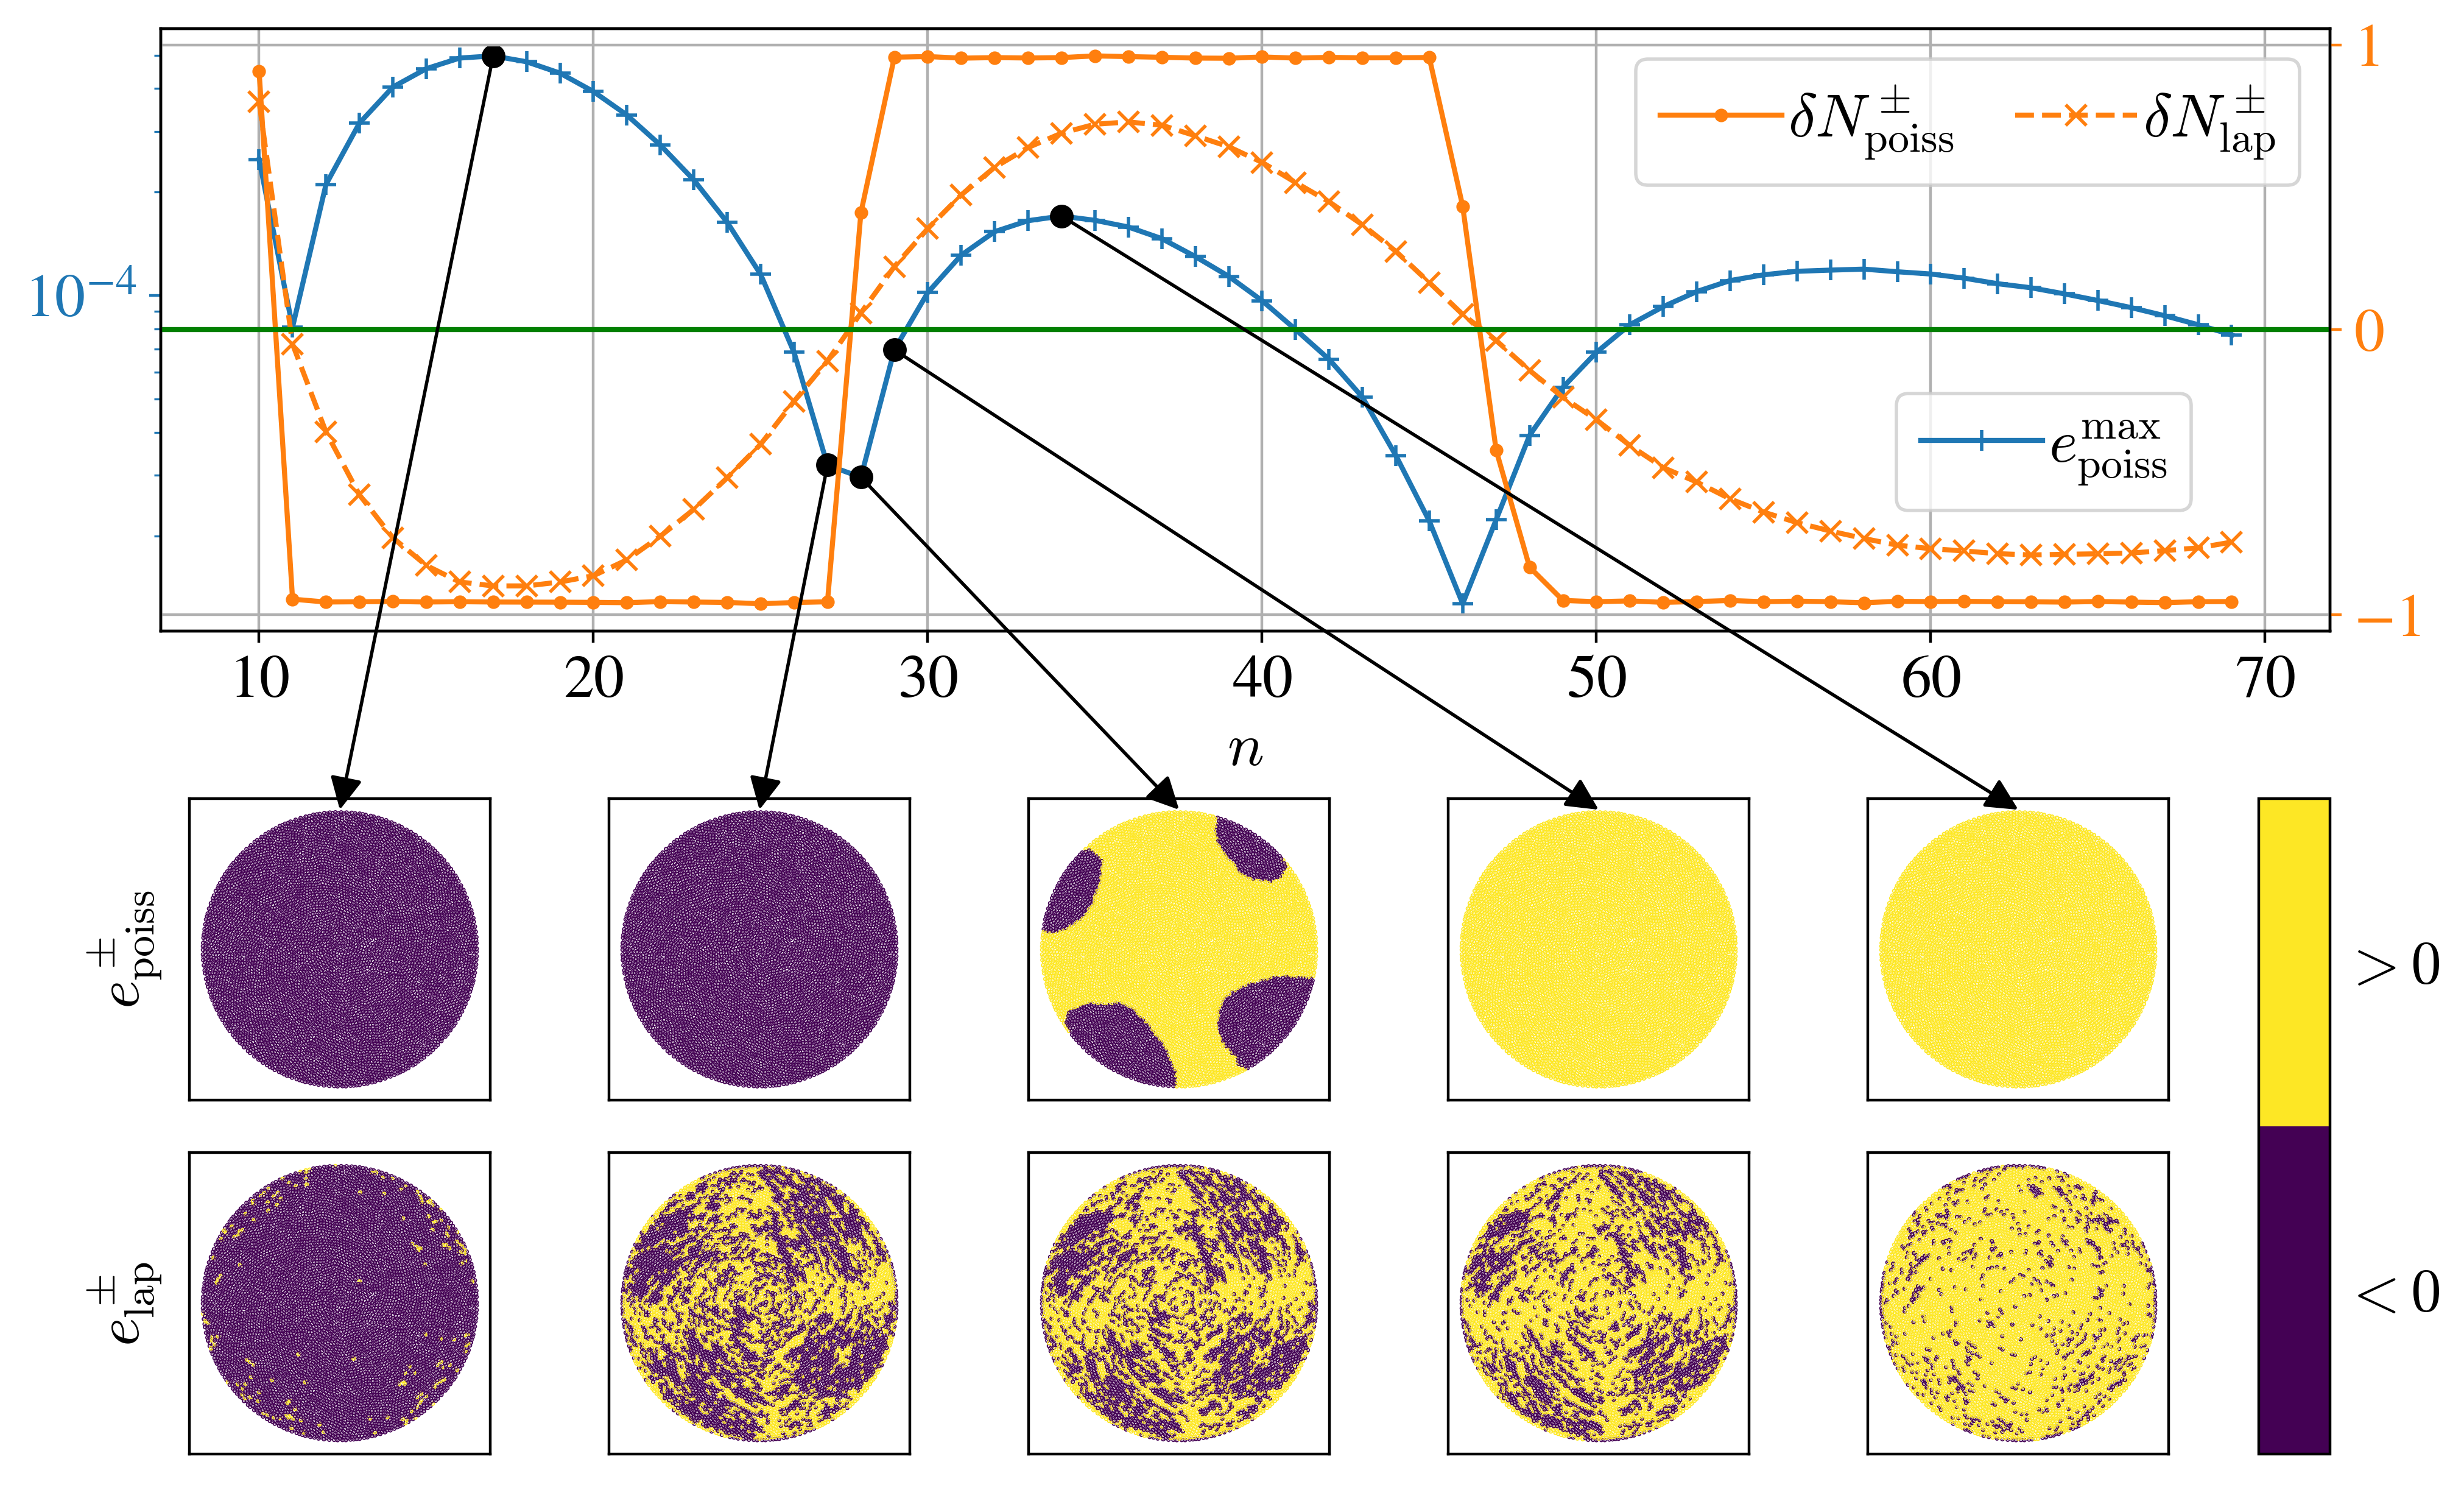
\includegraphics[width=.9\linewidth,center]{Figures/MetricContours.png}}
\end{frame}
\end{document}